\subsection{Sources of uncertainty}

In responce to increasing SST, the changes in climate tend to agree in a handful of observed ``convergence zones.''
Convergence zones are long and narrow bands of tropical convection anchored by SST structures.
These changes include a wet-get-wetter paradigm and a warmer-get-wetter mechanism, for uniform and projected SST increases, respectively.
The spatial pattern of SST change is the main driver of uncertainty between these two modes of precipitation change in the observed convergence zones.
SST change and preciptiation plotted over one another can be seen in Figure \ref{fig:148}.\\



\begin{figure*}[h!]
\begin{center}
  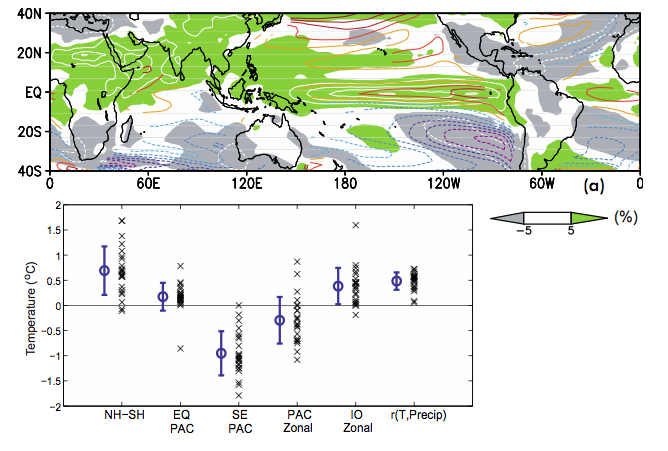
\includegraphics[width=0.790\textwidth]{fig148.png}
  \label{fig:148}
\end{center}
\end{figure*}


Over the tropical Atlantic, models agree poorly over current conditions due mainly to a northernly biased ITCZ and a cold tongue in (our) summer.
Models are able to capture the general warming trend over the past century in the Atlantic, but this results in a southward displaced Atlantic ITCZ.\\

Observational uncertainty, limited data, and changing measurement techniques all make the projection of zonal SST gradient difficult, and some models show strengthening while other models show weakening.
The ENSO variability over the past century is reproduced both in variability and spatial pattern by models with external forcing and without forcing, such that there is little agreement on whether external forming plays a role in the observed changes in ENSO.\\

Again due to uncertainties in SST projections, the ENSO spatial pattern change has low confidence.\\

\subsection{Agreement in convergence zones}

The three main convergence zones are the ITCZ, the South Pacific Convergence Zone (SPCZ), and the South Atlantic Covergence Zone (SACZ).\\
%%Of these, the IPCZ has known biases which are strongest in (our) summer, while the SPCZ and the SACZ model predictions generally agree over the past century.

The ITCZ suffers an unrealistic double-ITCZ pattern over the tropical Pacific and the Atlantic, which results in excessive rainfall over the southern flank.
This is due to the incorrect orientation of the SPCZ, missing the southeastward orientation of the SPCZ and aligning it with the ITCZ.
Changes in ENSO displace and change the orientation of the SPCZ as well, moving the SPCZ northeast and aligning it zonally in response to stronger events.
This shift to zonally-oriented SPCZ is consistent in both the CMIP3 and CMIP5 models, and increasing in frequency in the future.
This relies on a reduction in near-equatorial SST gradient, a consitent finding in response to human forcing.
A consistent shift of the SPCZ woudl result in major changes for the southwest Pacific, including potentially a longer dry spell.\\

In the SACZ, changes have a major impact on the precipitation over southeast South America.
The projected southward displacement and intensification will likely result in changes in the flood and dry conditions of South America, to which the current SPCZ pattern effects over Brazil.\\

\subsection{ENSO persistence}

Depsite the uncertainties in the spaital particularities of the ENSO, the amplitude modulation are well reproduced over the past century by models and the generation of the 10-100 year modulations by coupled GCM's without forcing.
Poor observations of the detailed coupled air-ocean feedbacks before 1970 make the discernment of forcings' role in ENSO uncertain, as mentioned earlier.\\

The improvement in the modelling of ENSO intensity from CMIP3 to CMIP5 is significant, and due to increased moisture with rainfall variability is expected to increase regionally.
Although the future changes in intensity are not confident due to the many factors on which ENSO depends, we remain very likely that this will continue to be the dominant mode of climate variability.
In Figure \ref{fig:1414} we can see how likely this is.\\

\begin{figure*}[h!]
\begin{center}
  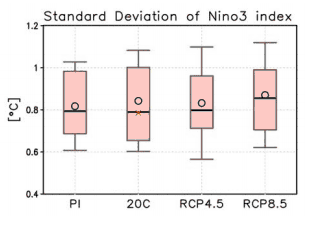
\includegraphics[width=0.490\textwidth]{figure1414.png}
  \caption{Standard deviation of Niño3 SST anomalies from CMIP5 model experiments.
    PI is the pre-industrial control experiment, 20C is the 20th Century control experiment, RCP4.5/8.5 are the 21st Century projections.
    The cross mark on 20C is the current observation.}
  \label{fig:1414}
\end{center}
\end{figure*}

\subsection{Future goals for Climate Scientists}

To make better predictions of the climate, we need to focus on our ability to reproduce the known large scale structures such as covergence zones that drive regional climate changes.
A better understanding of these structures, coupled with better observations, will allow us to ensure that the models accurately represent these structures togay and how they have changed during our observations, such that we can have confidence in future predictions.
In addition, the convergent structures drive regional precipitation patterns, which are economically and socially important outputs of climate modelling for the future. \\

A case study for this work has been the work of the past few decades on the ENSO.
Once poorly understood, it was foreseen by Charney and the vast amounts of work we have put forth to understand this phenomena have allowed us to be able to predict how it will change in the future.
Only with better observations, over a longer time, can we be more sure of the changes in intensity of these structures as well.\\






